% $Id: adjustment.tex 7816 2020-05-31 22:47:54Z mskala $

%
% MSK 013 testing and adjustment instructions
% Copyright (C) 2020  Matthew Skala
%
% This program is free software: you can redistribute it and/or modify
% it under the terms of the GNU General Public License as published by
% the Free Software Foundation, version 3.
%
% This program is distributed in the hope that it will be useful,
% but WITHOUT ANY WARRANTY; without even the implied warranty of
% MERCHANTABILITY or FITNESS FOR A PARTICULAR PURPOSE.  See the
% GNU General Public License for more details.
%
% You should have received a copy of the GNU General Public License
% along with this program.  If not, see <http://www.gnu.org/licenses/>.
%
% Matthew Skala
% https://northcoastsynthesis.com/
% mskala@northcoastsynthesis.com
%
\chapter{Adjustment and testing}

Most features of the Middle Path VCO should work to an acceptable standard
without requiring any adjustment; but the scale factor for the V/octave
inputs (also known as ``tracking'') and the shape of the sawtooth waveform
outputs each benefit from adjustment of the built-in trimmers as described
in this section.  I also give some suggestions on troubleshooting build
problems.

A multimeter is recommended for basic debugging.  An oscilloscope and an
accurate source of voltages are recommended for tracking and wave shape
adjustments.

\section{Short-circuit test}

With no power applied to the module, check for short circuits between the
three power connections on the Board~2 Eurorack power connector.  The first
pair of pins at the right, marked with white on the circuit board, are for
$-$12V.  The next three pairs are for 0V; and the next pair after that are for
$+$12V.  Check between each combination of these three voltages, in both
directions (six tests in all).  Ideally, you should use a multimeter's
``diode test'' range for this; if yours has no such range, use a low
resistance-measuring setting.  It should read infinite in the reverse
direction (positive lead to $-$12V and negative lead to each of the other
two, as well as positive lead to ground and negative to $+$12V) and greater
than 1V or 1k$\Omega$ in the forward direction (reverse those three tests). 
If any of these six measurements is less than 1k$\Omega$ or 1V, then
something is wrong with the build, most likely a blob of solder shorting
between two connections, and you should troubleshoot that before applying
power.

\emph{Optional}:  Although we test all cables before we sell them, bad
cables have been known to exist, so it might be worth plugging the Eurorack
power cable into the module and repeating these continuity tests across the
cable's corresponding contacts (using bits of narrow-guage wire to get into
the contacts on the cable if necessary) to make sure there are no shorts in
the cable crimping.  Doing this \emph{with the cable connected to the
module} makes it easier to avoid mistakes, because the module itself will
short together all wires that carry equal potential, making it easier to be
sure of testing the relevant adjacent-wire pairs in the cable.

Plug the module into a Eurorack power supply and make sure
neither it nor the power supply emits smoke, overheats, makes any unusual
noises, or smells bad.  If any of those things happen, turn off the power
immediately, and troubleshoot the problem before proceeding.

\section{Checking and adjusting wave shapes}

Apply power to the module and remove any other cables.  Set all the tuning
knobs and PWM knobs to the centres of their ranges, and set the sync switch
to the centre ``off'' position.  Use an oscilloscope to examine each of the
four output waveforms from the master oscillator and compare them with the
examples in Figure~\ref{fig:output-examples}.

\begin{figure*}
\centering\begin{tabular}{cc}
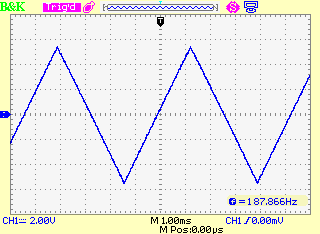
\includegraphics[scale=0.65]{bk3.png} & 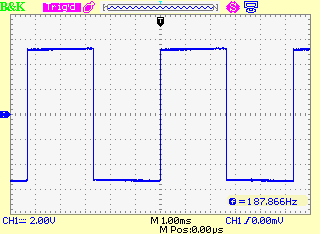
\includegraphics[scale=0.65]{bk5.png}\\
TRI & SQR \\
\strut & \\
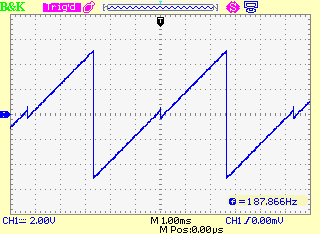
\includegraphics[scale=0.65]{bk4.png} & 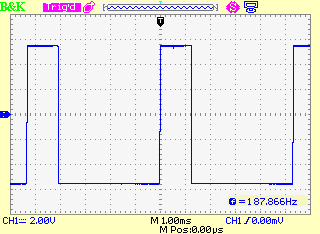
\includegraphics[scale=0.65]{bk6.png}\\
SAW & PULS
\end{tabular}\par
\caption{Output waveforms.}\label{fig:output-examples}
\end{figure*}

They should all look similar to the examples.  The exact frequency may be
different.  Try turning the master oscillator PWM knob and see that it
varies the duty cycle of the PULS waveform.

If the module is not already adjusted, the SAW waveform will probably have a
glitch or kink in it where it crosses zero, as shown in the figure.  Adjust
the SAW SHAPE A trimmer, which is on the back of the module in the upper
right quadrant of the board, to minimize this kink.  There will probably
always be a small ultrasonic spike in the waveform at this point, but you
should be able to get the straight segments on either side to align well
with each other.

Repeat these checks for the slave oscillator, and adjust the SAW SHAPE B
trimmer, at the centre left of the board, to make the slave SAW shape as
good as possible.

\section{Checking the sine shaper}

This test is not absolutely necessary, but it provides an easy way of
checking the operation of the sine shaper.  It will require an oscilloscope
capable of X--Y display mode.

Turn the coarse and fine tuning knobs for one of the oscillators to about
1~o'clock, that is, a little higher than midpoint.  Turn off sync.  Turn the
shaper knob for that oscillator to maximum (fully clockwise) and the other
two shaper knobs to zero (fully counterclockwise).  Use the TRI output for
the oscillator as the horizontal input (X coordinate) for your oscilloscope
and connect each of the three sine shaper outputs to the vertical, in turn. 
Compare the display with the examples in Figure~\ref{fig:shaper-samples}.

\begin{figure*}
\centering\begin{tabular}{cc}
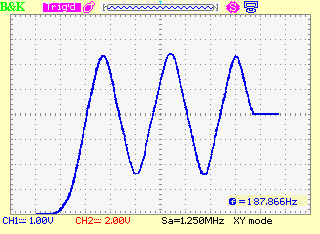
\includegraphics[scale=0.65]{bk7.png} & 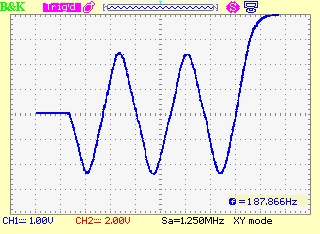
\includegraphics[scale=0.65]{bk9.png}\\
sin & cos \\
\strut & \\
\multicolumn{2}{c}{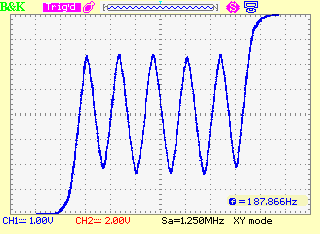
\includegraphics[scale=0.65]{bk8.png}}\\
\multicolumn{2}{c}{both}
\end{tabular}\par
\caption{Sine shaper voltage functions.}\label{fig:shaper-samples}
\end{figure*}

In this test setup, the oscilloscope display represents the voltage function
computed by the shaper.  Each result should look a lot like the examples;
there may be some small variation in the height or spacing of the peaks.  If
there is a significant difference from the examples, such as a peak much
higher or lower than the others or missing entirely, it suggests a problem
in the shaper, most likely with one of the transistors; see the
``Troubleshooting'' section below.

\section{Tracking (with automated test)}

``Tracking'' refers to the slope of the V/octave control voltage response. 
It should be exactly 1.0V/octave.  The trimmers R10 and R46, located on
Board~1, adjust this response for the master and slave oscillators
respectively.

The best way to adjust this setting, if you have the equipment and
skills, is by hooking up the module to a computer that can send it control
voltages, measure the output frequency in self-oscillation, and compute an
estimate of the current V/octave ratio, which allows realtime feedback as
you adjust the trimmer.  I provide a piece of software in the file
\texttt{voct-0.1.tar.gz} to support this process.

The software is written for the Linux ALSA MIDI and PCM drivers, and it
includes hardcoded assumptions about things like device numbers.  \emph{You
need C programming skills to use this software.  I will not provide
support on it.}  If you cannot modify the software as needed to suit your
installation, then I recommend using the manual tracking procedure in the
next section instead.

Read the C source code and make any appropriate changes for your
installation.  Compile it.  Connect your MIDI-to-CV interface to the V/oct
input on one oscillator of the MSK~013, and connect the SQR output to your
computer's audio input (with attenuation, if required).  Remove any other
patch cables from the MSK~007.  Optionally (requires other appropriate
software, not included), send MIDI note 69 to the MIDI interface and adjust
the tuning of the MSK~013 to make it oscillate at 440Hz; otherwise set the
coarse tuning to about 10 o'clock and the fine to its midpoint.  Adjut the
sensitivity of the audio input, or the attenutation if you are using an
attenuator, to bring the Leapfrog's signal to about 50\%\ of full scale. 
Run the \texttt{vcoslope} software.

The vcoslope program sends random MIDI notes, makes brief recordings of the
oscillator output, and attempts to fit an exponential function (using linear
regression) to the note/frequency data in the last $N$ notes, for several
different values of $N$.  From that it can determine the current sensitivity
of the V/octave input.  Using multiple frequencies to test like this gives
better accuracy than would be the attainable with just testing at two
frequencies (as in the standard manual procedure).  Using notes in random
order is preferable to testing them in an increasing or decreasing sequence,
because of self-heating effects in the exponential converter.  The program
tries multiple sample sizes (the most recent 10, 32, 100, and 316 points)
to allow both quick feedback on any trim changes, and accurate results over
longer periods.

It will start producing lines of output, one every few seconds.  Each
line starts with a decimal sequence number (1, 2, 3, \ldots) and the MIDI
note number that was sent.  The next two columns are the measured frequency
in Hertz, and the number of octaves plus or minus that is relative to the
440Hz reference pitch.  Then come up to four columns of V/octave estimates:
the first determined from the last 10 notes tested, the second from the last
32 notes, then 100 notes, then 316 notes.  These columns each show up only
once there have been the requisite number of notes, so at first there will
be no such column, then the first one will appear on the tenth note, then
the second at note 32, and so on.

Let the program run for at least 10 or 20 notes so you can get some idea of
the module's current V/octave response.  Then try adjusting the trimmer one
turn clockwise.  Watch for another 10 lines of output.  The 10-note V/oct
estimate should start to move, then settle in on a new value.  From there
you should be able to estimate how far (how many turns) and in which
direction you need to adjust the trimmer to bring the response to
1.000V/oct.  Try to do that.  As you get in closer, the natural noise in the
V/oct numbers may become significant in relation to the sizes of adjustment
you are making.  In that case, switch to one of the slower-updating columns
to get a more stable reading (larger sample size).  You will need to wait
longer between adjustments for those columns to reach full precision. 
Continue until you have the module performing as accurately as you want, or
until you run out of patience.

Repeat the process for both oscillators.  When adjusting the slave, make
sure sync is turned off.

\section{Tracking (by hand)}

This simpler tracking procedure does not require computer skills, only the
ability to send reproducible control voltages of 0V and 1V to the module and
test the resulting frequencies.  It is somewhat less accurate because it
tests only two frequencies instead of averaging over many, but most DIY VCOs
are routinely adjusted this way.

A North Coast Synthesis MSK~008 Octave Switch, assuming it has itself been
properly adjusted, makes an ideal voltage source for the following
procedure.

Hook up your control voltage source to the oscillator's V/oct input, set up
your equipment as necessary to test the frequency of one oscillator output,
disconnect any modulation signals, and power up the module.

Send a 0V control voltage to the oscillator.  Tune it with the coarse and
fine tuning knobs to an oscillation frequency of 220Hz (or any arbitrary
frequency of your choice, but this one is convenient).

\emph{Without changing the tuning knob settings,} send a 1V control voltage
to the oscillator.  Adjust the trimmer, not the tuning knobs, to bring the
oscillation frequency to 440Hz (or twice the initial frequency if you are
using something other than 220Hz).

Send a 0V control voltage and test the output frequency; is it 220Hz or your
chosen other reference frequency?  If not, adjust the tuning knobs to make
it so.  Repeat these two steps, of alternately adjusting for the low
frequency with 0V and the tuning knobs, and the high frequency with 1V and
the trimmer potentiometer, until both readings are reliably what they should
be without seeming to need further adjustment.

For even better accuracy:  use two control voltages more than 1V apart, and
a correspondingly wider frequency range.  For instance, an MSK~008 Octave
Switch can conveniently
generate $+$1V and $-$1V, which could be used with reference frequencies of
440Hz and 110Hz to set tracking over two octaves instead of just one.

\section{Troubleshooting}

If the module does not perform as it should, some kind of debugging or
troubleshooting may be necessary.
It would require several books to convey all the skills and knowledge useful
in troubleshooting even a simple electronic circuit like this one, but here
are some possible symptoms and some suggestions on diagnosis and treatment.

In general, the first order of business in debugging is to narrow down the
set of things that could be wrong.  Think about the different sections of
the module:  master oscillator, slave oscillator, sine shaper, sync, power
system.  Any single problem is likely to involve at most one of those,
although it is also possible for there to be more than one independent
problem occurring at once.  If you can determine which of those large
sections is at fault, try to narrow it down further:  does the problem
affect just one output?  Just one input?  Is it limited to a specific
feature of the module?  The more narrow a description you can find, the
fewer places you will have to look to find out what is wrong.

No response from the module at all:  This module should produce some output
from each oscillator's TRI, SQR, and SAW jacks (at least) at all times
regardless of the knob and switch settings, so if there is no such output it
suggests a power problem, such as a power cable plugged in wrong or a short
circuit.  This might even be a problem in the power supply and not the
module itself.  If possible, check the power supply with some other load
instead of the new module to rule out the power supply itself as the
location of the problem.

General quality issues:  many problems can be diagnosed just by looking
closely at your work, preferably with at least one night's sleep between
when you assembled the module and when you examine it.  Look for bad solder
joints that fail to connect; solder bridges between nearby connections
(especially on the discrete transistors in the sine shaper);
components missing; components exchanged (especially resistors with similar
colour codes, such as 1k$\Omega$ swapped with 10k$\Omega$); polarized
components such as diodes mounted backwards; and so on.

General tips for debugging DIP ICs:  make sure for, for each IC, that
\begin{itemize}
  \item it really is the type of IC it's supposed to be, not something else
    (beware of cheap ICs you buy from Chinese sellers on eBay and
    AliExpress, especially if they are offering unusually good prices on
    expensive chips like the AD633);
  \item it is plugged in snugly;
  \item all the legs of the chip go nicely into the corresponding holes in
    the socket, with none bent outside or folded up under the chip;
  \item it is plugged in \emph{at all} (forgetting to do so is a surprisingly
    common mistake!);
  \item it is plugged in the right way around, with the Pin~1
    indentation or notch matching the clues on the
    board (if this is wrong, the chip is probably destroyed and will need to
    be replaced);
  \item there are no solder bridges on the chip socket, unsoldered pins,
    debris clogging the socket holes, or similar; and
  \item its decoupling capacitors (the small ceramic ones) are installed and
    there is nothing wrong with their solder joints.
\end{itemize}

You can try swapping a suspect chip with another one of the same type from
elsewhere in the module and see if that causes the problem to change; if so,
it's likely one of the two you swapped was bad.

No signal coming out of one jack, or no response to
input on one jack:  make sure that a signal or a response is expected based
on the other settings of the module, but if so, this suggests a bad jack. 
During prototyping I had some problems with jacks that had been
overenthusiastically soldered, warping their plastic bodies so that they
shorted out when receiving plugs.  If possible, try wiggling the plug in the
jack, and try inserting it and removing it slowly, watching the response. 
If it works with the plug inserted just partially, but not when fully
inserted, that suggests a damaged jack.

Bad wave shapes:  Each oscillator output comes from the core and passes
through at least a little bit of circuitry unique to that output.  If the
problem shows up in just one waveform, it is probably in the amplifier or
shaper for that one output.  If it affects multiple outputs, it's more
likely a problem with the cores.  Consult the schematic to figure out which
ICs are relevant to the problem you're seeing, and check those ones first. 
One syndrome I've noticed is that a bad MOSFET in the sawtooth shaper
(which could be defective to begin with; damaged by static or by soldering
heat; or subjected to a solder bridge) tends to lead to a slanted-topped
square wave instead of a sawtooth on the SAW output.

Exponential converter troubles:  some parts of the exponential converter are
shared between the two oscillators, so if there are serious problems with
tracking or modulation affecting \emph{both} oscillators, it points to an
issue with those shared components (the THAT320 and reference current
generators).  On the other hand, an issue with the tracking or modulation
affecting only one of the two oscillators is likely to be in the parts
specific to that one oscillator.

Sine shaper problems:  one of the most common build issues with this module
is for a transistor in the sine shaper to be badly soldered, causing it to
either conduct when it shouldn't, or fail to conduct when it should.  Since
each of these transistors is meant to turn on at a different input voltage,
it's possible to locate which transistor is bad by figuring out at which
voltage the problem shows up.  Each positive and negative peak in the
voltage curves corresponds to one transistor.  If you measure the voltage
curves (as described under ``Checking the sine shaper'' above) and they do
not match the examples, consult the idealized curves in
Figures~\ref{fig:shaper-sincos} and~\ref{fig:shaper-both}, in which each
peak is labelled with the name of the transistor responsible for it.  Half
the transistors contribute to each of the ``sin'' and ``cos'' outputs, and
all transistors contribute to the ``both'' output.  The transistor named at
whatever part of the curves seems not to match the examples, is the one you
should check first as a possible source of the trouble.

\begin{figure*}
\centering
\includegraphics[scale=1.15]{sin.pdf}\par
\includegraphics[scale=1.15]{cos.pdf}\par
\caption{Voltage functions for ``sin'' and ``cos'' outputs.}\label{fig:shaper-sincos}
\end{figure*}

\begin{figure*}
\centering
\includegraphics[scale=1.15]{both.pdf}\par
\caption{Voltage function for ``both'' output.}\label{fig:shaper-both}
\end{figure*}

